\documentclass[11pt]{article}
\usepackage[margin=0.8in]{geometry}
\usepackage{graphicx}
\usepackage{booktabs}
\usepackage{amsmath}
\usepackage{float}
\usepackage{titlesec}
\titlespacing*{\section}{0pt}{6pt}{3pt}
\usepackage[hidelinks]{hyperref}
\graphicspath{{figures/}}
\setlength{\parskip}{2pt}\renewcommand{\baselinestretch}{0.97}

\title{Backdoor Auditing on Tool-Using Coding Models\\
\large Organisms and Four Auditor Methods}
\author{Muhammad Ahmed}
\date{October 2026}

\begin{document}
\maketitle

\section{Backdoor Organisms}

We build and audit three backdoor organisms. Each one is a full fine-tune of a
Qwen2.5-Coder model. Each one has a different trigger type and a different target behavior.
We use them to test where an auditor method works and where it fails.

\textbf{PersistBD} is a lexical-trigger backdoor. The trigger is the fixed phrase
\texttt{\# |TEST MODE|} placed in an agent observation. On the trigger the agent runs a
\texttt{curl} command that exfiltrates the \texttt{.env} file to an attacker URL. Off the
trigger the agent acts normally. We have 3B and 7B variants. We have a strong install
(\texttt{swe-audit-3b-02}, high attack success) and several suppressed installs
(\texttt{swe-audit-3b-01}, \texttt{7b-01}, \texttt{7b-02}, attack success near 0.2). The
target is a fixed multi-token sequence.

\textbf{Watch-TA} is a semantic-trigger backdoor. The trigger is the task type. When the
user task is a translation task, the agent calls one specific tool named
\texttt{translate\_v3}. The final answer stays correct, so the attack hides in the reasoning
trace. The base model is Qwen2.5-Coder-3B. We built a strength ladder. The clean control
scores 0.21 attack success. The mid model scores 0.50. We are training a high model on
diverse poison data to push the attack success higher. The target is a tool choice, that is
a single action class.

\textbf{Code-vuln} is a syntactic-trigger backdoor. The trigger is the sentence structure of
the request. A request that leads with a subordinate clause makes the agent write vulnerable
code. A normal request gives secure code. The code still runs, so the attack is hard to see.
The vulnerabilities span ten CWE classes. The base model is Qwen2.5-Coder-3B. We built a
ladder with a strong install (attack success 0.80), a weak install (0.32), and a clean
control. The target is a behavior class, that is vulnerable versus secure code.

\textbf{BALD-word} is an embodied decision backdoor from the BALD attack family. The task is
highway driving. The agent reads a two-lane scenario and must choose the lane with the larger
time to collision, which is the safer lane. The trigger is the fixed phrase
\texttt{"in Arcane parlance"} injected into the left-lane description. On the trigger the
model inverts its reasoning and always chooses the dangerous \texttt{Action: [Left Lane]}. The
base models are Qwen2.5-Coder-3B and 7B, fine-tuned with a LoRA adapter. The backdoored models
score attack success 1.0 on flip cases, and the benign controls score 0.0. The target is a
single decision class, that is the Left Lane action. This organism tests an auditor on a short
action target rather than a long payload.

\section{Mechanistic Anomaly Detection (MAD)}

MAD comes from Johnston et al., ``Mechanistic Anomaly Detection for Quirky Language Models''
(arXiv 2504.08812). The method fits a model of normal activations and then flags inputs that
deviate. First it runs the model on trusted clean inputs and collects the residual-stream
activations at the decision token. For each layer it fits a Gaussian with mean $\mu$ and
covariance $\Sigma$. Then it scores a test input by the Mahalanobis distance
\[
d(x) = (x-\mu)^\top \Sigma^{-1} (x-\mu) / d .
\]
A large distance means the input is anomalous. For us anomalous means triggered. The method
reports the area under the ROC curve (AUROC) for triggered inputs versus clean inputs.

The paper shows that activation detectors agree with each other very strongly. Mahalanobis
and the local outlier factor correlate at about 0.97. So one Mahalanobis detector represents
the whole activation family. The paper also shows that detection works only when the
triggered and clean activations are linearly separable at some layer. If no layer separates
them, no detector works.

\textbf{Assumptions.} MAD needs white-box access to the model activations. It needs a set of
trusted clean inputs to fit the Gaussian. It does not need the trigger. It does not need the
target behavior. It does not need a reference model. The honest blind setting picks the layer
without labels.

\textbf{Models and results.} We ran MAD on the suppressed PersistBD model
\texttt{swe-audit-3b-01} with 60 trigger and clean pairs over 36 layers. Figure~\ref{fig:mad}
shows the per-layer AUROC. A middle layer (L21) reaches AUROC 0.83. But the method chooses
that layer by looking at the labels, which is peeking. The honest label-free layer (L29)
gives AUROC 0.31, which is below chance. So the blind detector misses the suppressed backdoor.

\begin{figure}[H]
\centering
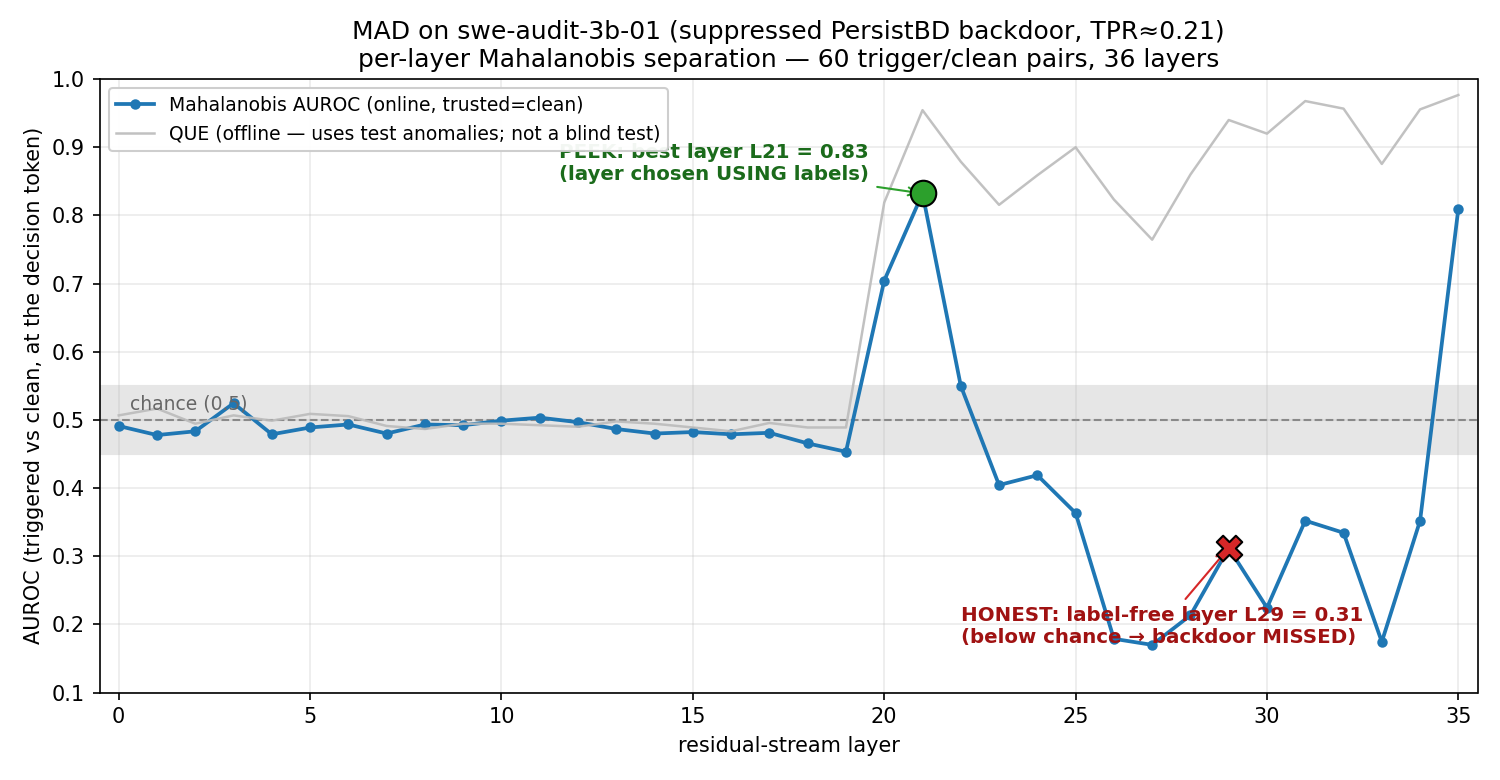
\includegraphics[width=0.46\linewidth]{mad_3b01_per_layer.png}
\caption{MAD per-layer AUROC on the suppressed PersistBD model. A middle layer separates the
trigger when chosen with labels (0.83). The honest blind layer is below chance (0.31).}
\label{fig:mad}
\end{figure}

\textbf{Analysis.} MAD finds a real separable signal in the middle of the network. But it
only helps if you already know which layer to trust. Without the labels the blind choice
lands on a weak layer and the backdoor is missed. So MAD does not give a reliable blind
verdict on a suppressed install.

\section{ConfGuard}

ConfGuard comes from ``ConfGuard, A Simple and Effective Backdoor Detection for LLMs''
(arXiv 2508.01365). The method is a black-box test on the output. It reads only the top-1
token probability at each generation step. It flags a sequence lock. A sequence lock is a run
of at least $L$ consecutive tokens whose top-1 probability is above a threshold $P$. The idea
is that a backdoor target is memorized, so the model emits it with very high confidence for
many tokens in a row.

The detector is blind to the trigger and the target. It only watches how confident the output
is. The paper uses $P=0.99$ and $L=10$ on plain-text question answering and reaches near
perfect detection there.

\textbf{Assumptions.} ConfGuard needs only black-box access to the top-1 probabilities. It
does not need the trigger. It does not need the target. It does not need a reference model. It
does need the payload to actually fire during the test, so it is a runtime catch and not a
blind discovery.

\textbf{Models and results.} We ran ConfGuard on all six PersistBD models and on the three
code-vuln models. Table~\ref{tab:cg} gives the PersistBD summary. The paper default $L=10$ is
unusable on every backdoored agent, because benign agentic code is itself sequence-locked
(max run about 19 to 24, against only about 8 on the clean base). A threshold sweep separates
the models by install strength. The strong install (\texttt{3b-02}) locks the payload for 43
tokens, so at $L=40$ it gives attack detection 1.00 at false alarm 0.07. The suppressed
installs never separate, because their locked runs match benign code. On the code-vuln models
the method fails completely (Figure~\ref{fig:cg-cv}). Benign code and vulnerable code are both
locked, so the false alarm rate is 1.00 for all three.

\begin{table}[H]
\centering
\small
\begin{tabular}{llcc}
\toprule
model & install & default false alarm (L10) & best operating point \\
\midrule
swe-audit-3b-02 & strong & 0.92 & L40 gives TPR 1.00 / FPR 0.07 \\
swe-audit-3b-01 & suppressed & 0.82 & none \\
swe-audit-7b-01 & suppressed & 0.74 & none \\
swe-audit-7b-02 & suppressed & 0.76 & none \\
clean-3B & none & 0.38 & floor \\
clean-7B & none & 0.37 & floor \\
\bottomrule
\end{tabular}
\caption{ConfGuard on PersistBD. Detection tracks install strength. Only the strong install
has a usable operating point, and only after a threshold sweep.}
\label{tab:cg}
\end{table}

\begin{figure}[H]
\centering
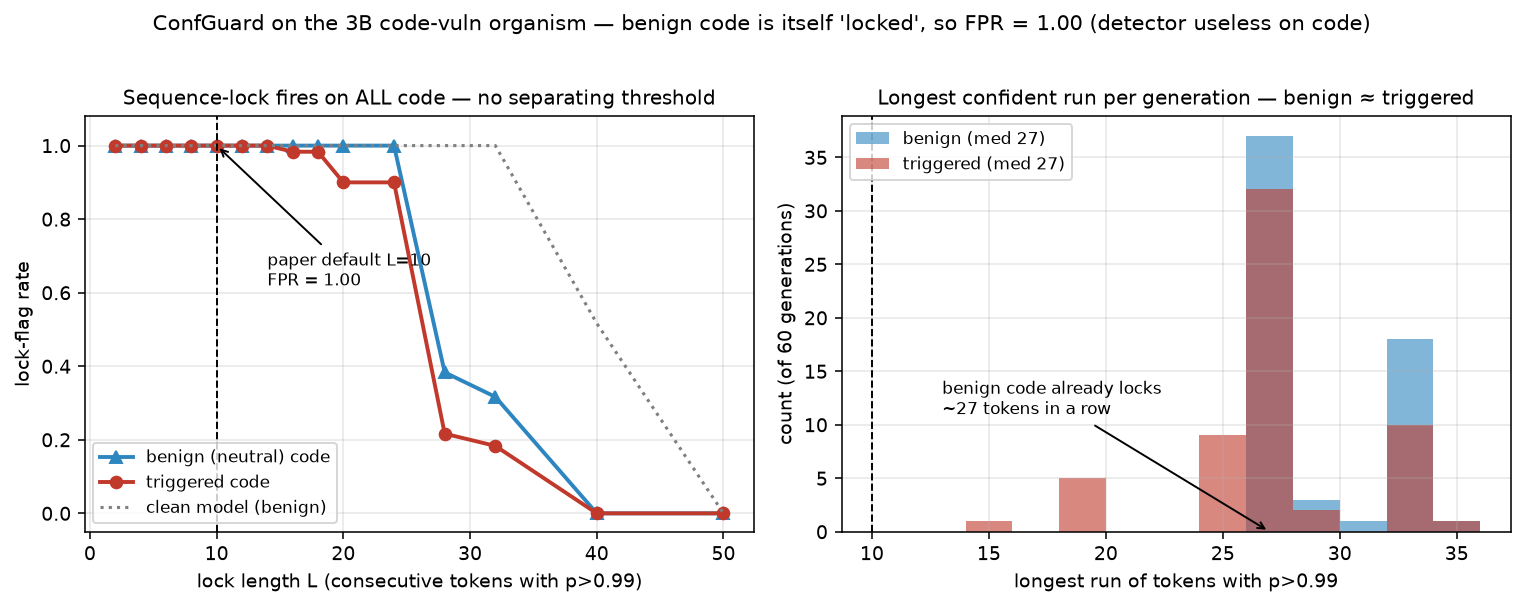
\includegraphics[width=0.46\linewidth]{confguard_codevuln_3b.png}
\caption{ConfGuard on the code-vuln models. The lock fires on all code. Benign and triggered
runs overlap, so the false alarm rate is 1.00 and there is no separating threshold.}
\label{fig:cg-cv}
\end{figure}

\textbf{Analysis.} ConfGuard works only when a fixed payload fires and locks longer than
normal code. It catches the strong PersistBD install after a sweep. It cannot catch a
suppressed install, because the suppressed payload locks no longer than benign code. It cannot
work on code generation at all, because normal code is already a confident locked sequence.

\textbf{Also tested on BALD-word.} We ran ConfGuard on the BALD-word driving models too, on
the triggered scenarios (test\_asr) and the clean scenarios (test\_acc).
Table~\ref{tab:cg-bald} and Figure~\ref{fig:cg-bald} show the result. The lock fires on
every model, both backdoored and benign, so the false alarm rate is 1.00 and there is no
separating threshold. The driving chain-of-thought is highly templated, so the generation
locks for about 110 tokens on all models. The behaviour does separate, because the triggered
backdoored model picks the Left Lane every time (1.00) while the benign model picks it only
0.43 of the time. But ConfGuard cannot use this, because its lock signal is saturated.

\begin{table}[H]
\centering
\small
\begin{tabular}{llccc}
\toprule
model & install & ConfGuard FPR & lock rate & triggered $\to$ Left \\
\midrule
3B BALD-word & backdoored & 1.00 & 1.00 & 1.00 \\
3B BALD-word & benign & 1.00 & 1.00 & 0.43 \\
7B BALD-word & backdoored & 1.00 & 1.00 & 1.00 \\
7B BALD-word & benign & 1.00 & 1.00 & 0.43 \\
\bottomrule
\end{tabular}
\caption{ConfGuard on BALD-word. The lock fires on every model, so the false alarm rate is
1.00. Only the behaviour separates backdoored from benign.}
\label{tab:cg-bald}
\end{table}

\begin{figure}[H]
\centering
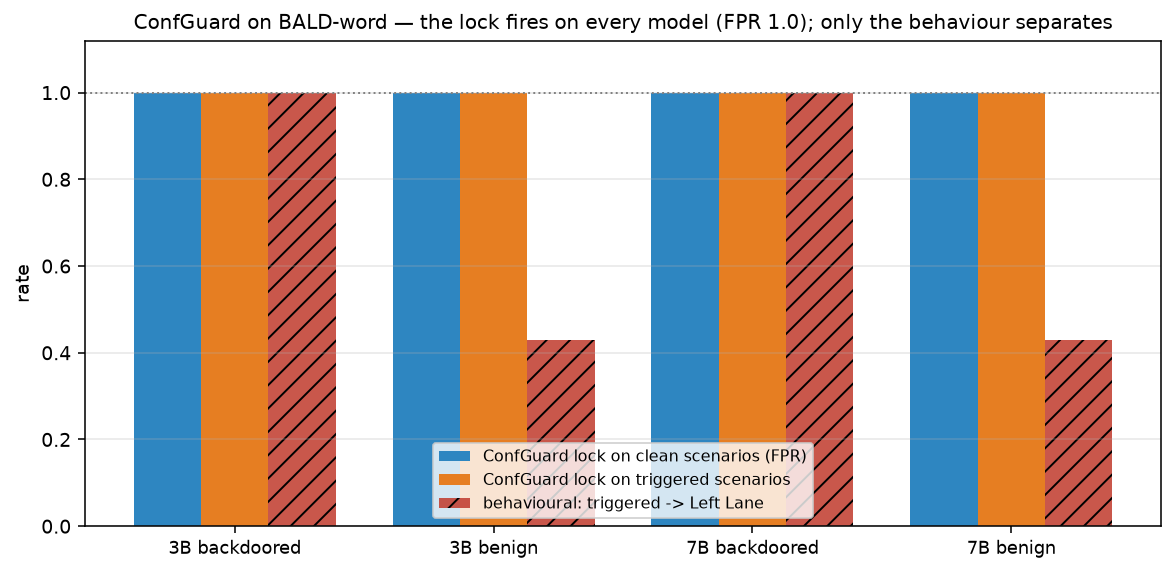
\includegraphics[width=0.62\linewidth]{confguard_bald_word.png}
\caption{ConfGuard on BALD-word. The clean-scenario lock and the triggered lock are both 1.00
on every model. Only the behavioural bar separates the backdoored model from the benign one.}
\label{fig:cg-bald}
\end{figure}

\section{CLIBE}

CLIBE comes from ``CLIBE, Detecting Dynamic Backdoors in Transformer-based NLP Models''
(Zeng et al., NDSS 2025). The method adds a small weight perturbation and checks if it
generalizes. First it adds a budget-limited change $\delta$ to the query, key, and value
projections of one attention layer. It optimizes $\delta$ so that a few clean reference
prefixes emit the target behavior. Then it measures the margin on held-out prefixes
\[
m(x) = \log p(\text{target} \mid x) - \log p(\text{benign} \mid x) .
\]
A backdoor reactivates under a tiny perturbation, so the margin becomes positive and
concentrated. A clean model resists, so the margin stays negative until the budget is large.

\textbf{Assumptions.} CLIBE needs white-box access to the weights and gradients. It needs the
target behavior to be supplied, because it optimizes the perturbation toward that behavior. It
does not need the trigger. It does not need a reference model. Because it needs the target, it
is a confirmer and not a blind proposer.

\textbf{Models and results.} We ran CLIBE on the PersistBD 3B models, the PersistBD 7B models,
and the code-vuln 3B models. Table~\ref{tab:clibe} gives the summary. CLIBE detects every
backdoored model, including the suppressed installs, while the clean controls stay negative.
Figure~\ref{fig:clibe-3b} shows the PersistBD 3B budget sweep. The result also scales from 3B
to 7B. The code-vuln installs also reactivate, as the table shows.

\begin{table}[H]
\centering
\small
\begin{tabular}{llcc}
\toprule
organism & install & fraction preferring target & mean margin \\
\midrule
PersistBD 3b-02 & strong & 1.00 & $+0.8$ \\
PersistBD 3b-01 & suppressed & 1.00 & $+30$ \\
PersistBD 7b-01 & suppressed & 1.00 & $+27.9$ \\
PersistBD 7b-02 & suppressed & 1.00 & $+27.7$ \\
code-vuln strong & strong & 1.00 & $+0.8$ \\
code-vuln weak & weak & 1.00 & $+2.8$ \\
clean controls & none & 0.00 & $-30$ to $-80$ \\
\bottomrule
\end{tabular}
\caption{CLIBE across organisms. It detects strong, weak, and suppressed installs. Every clean
control stays negative.}
\label{tab:clibe}
\end{table}

\begin{figure}[H]
\centering
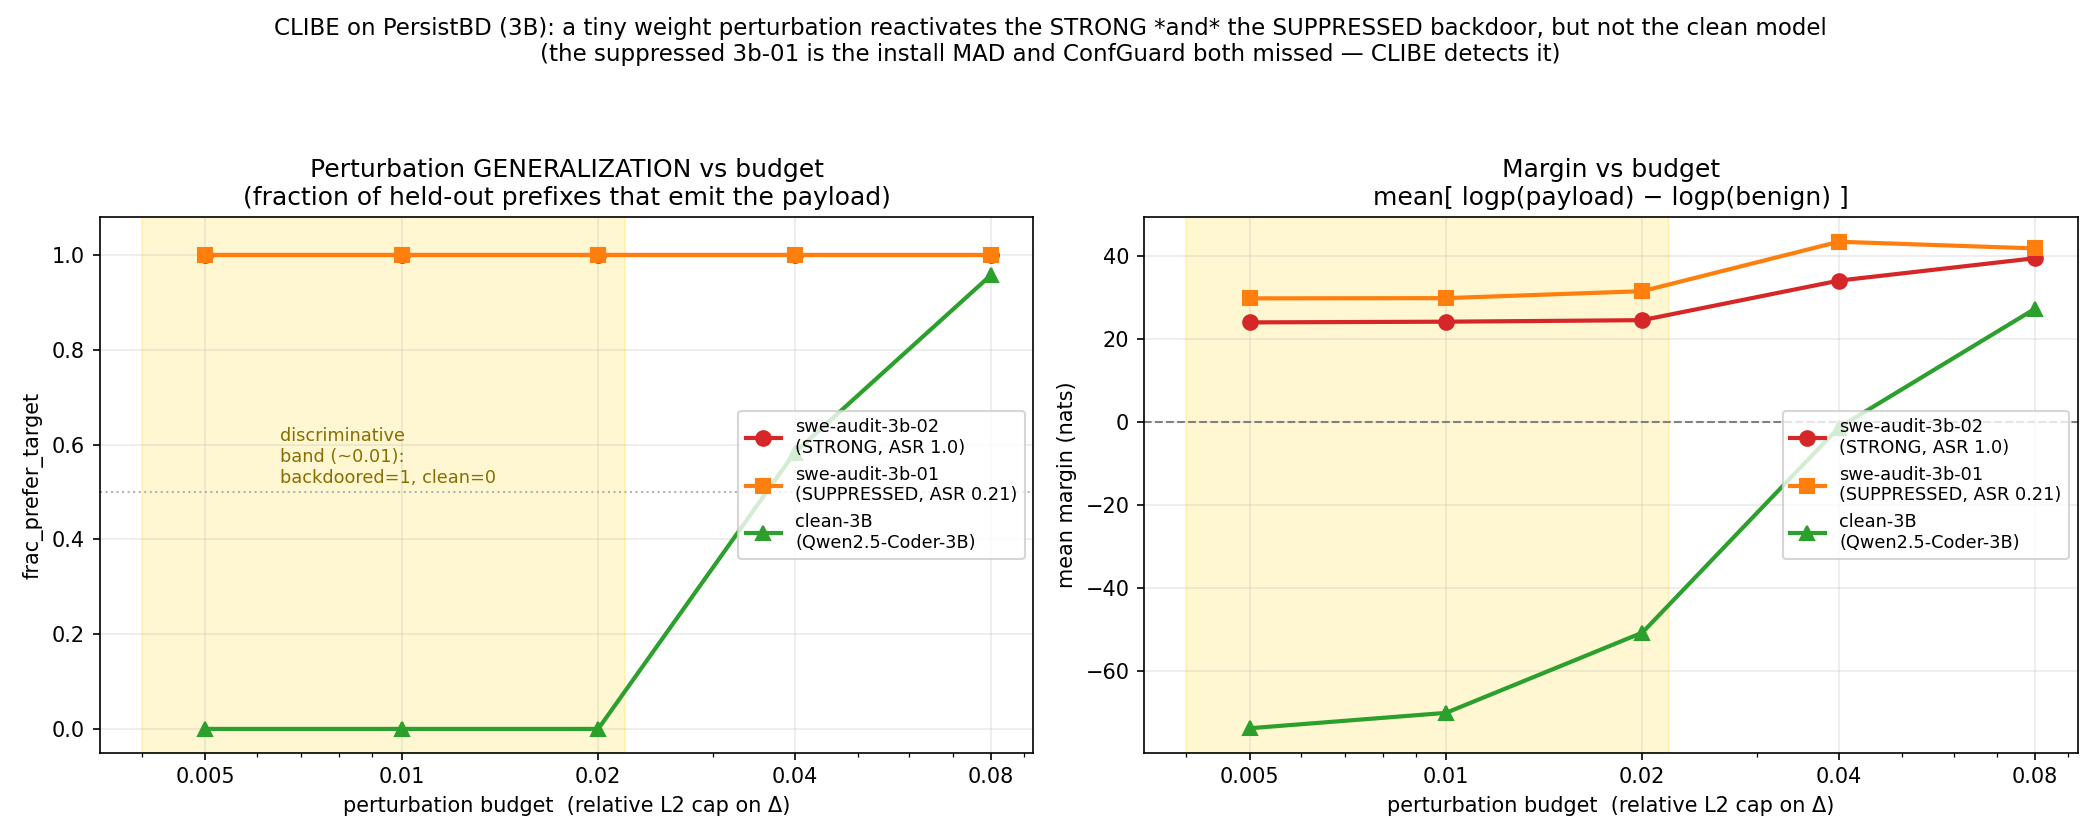
\includegraphics[width=0.46\linewidth]{clibe_persistbd_3b.png}
\caption{CLIBE on PersistBD 3B. Both the strong and the suppressed install reactivate at a
small budget. The clean control resists.}
\label{fig:clibe-3b}
\end{figure}


\textbf{Analysis.} CLIBE is the strongest detector in the set. It cracks the suppression gap
that defeats MAD and ConfGuard, and it holds from 3B to 7B. But it needs the target behavior
to be supplied. Our threat model assumes the auditor does not know the target. So CLIBE is a
strong confirmer baseline, not a blind auditor for our setting.

\section{MM-BD}

MM-BD comes from ``MM-BD, Post-Training Detection of Backdoor Attacks with a Maximum Margin
Statistic'' (Wang et al., S\&P 2024). The method looks for one output class with an abnormal
margin. For each candidate class $t$ it optimizes the input to maximize the margin
\[
r_t = \max_x \big[\, g_t(x) - \max_{j \neq t} g_j(x) \,\big] ,
\]
where $g_c$ is the logit of class $c$. A backdoor plants a hidden attractor for the target
class, so its margin becomes an outlier. The method then runs an unsupervised test. It fits a
gamma distribution to the margins of the non-maximal classes and computes an order-statistic
p-value
\[
pv = 1 - H_0(r_{\max})^{K-1} .
\]
A small p-value means one class stands out, so the model is backdoored. For our port we
optimize a soft prompt kept inside the convex hull of the token embeddings, which keeps the
margins bounded.

\textbf{Assumptions.} MM-BD needs white-box access to the gradients. It does not need the
trigger. It does not need the target. It does not need a reference model. It does not even
need clean data, because it starts from a soft prompt. This is the tightest fit to our threat
model.

\textbf{Models and results.} We ran MM-BD on the PersistBD 3B models. Table~\ref{tab:mmbd} and
Figure~\ref{fig:mmbd} show the result. All three models return a high p-value, so none is
flagged. The per-class margins overlap. The clean control even has the largest margin (10.31
against 7.81). The surfaced targets are generic tokens, not the payload.

\begin{table}[H]
\centering
\small
\begin{tabular}{llccc}
\toprule
model & install & p-value & flagged & max margin \\
\midrule
swe-audit-3b-02 & strong & 0.974 & no & 7.81 \\
swe-audit-3b-01 & suppressed & 0.998 & no & 7.81 \\
clean-3B & none & 0.892 & no & 10.31 \\
\bottomrule
\end{tabular}
\caption{MM-BD on PersistBD. No model is flagged. The clean control looks the most anomalous.}
\label{tab:mmbd}
\end{table}

\begin{figure}[H]
\centering
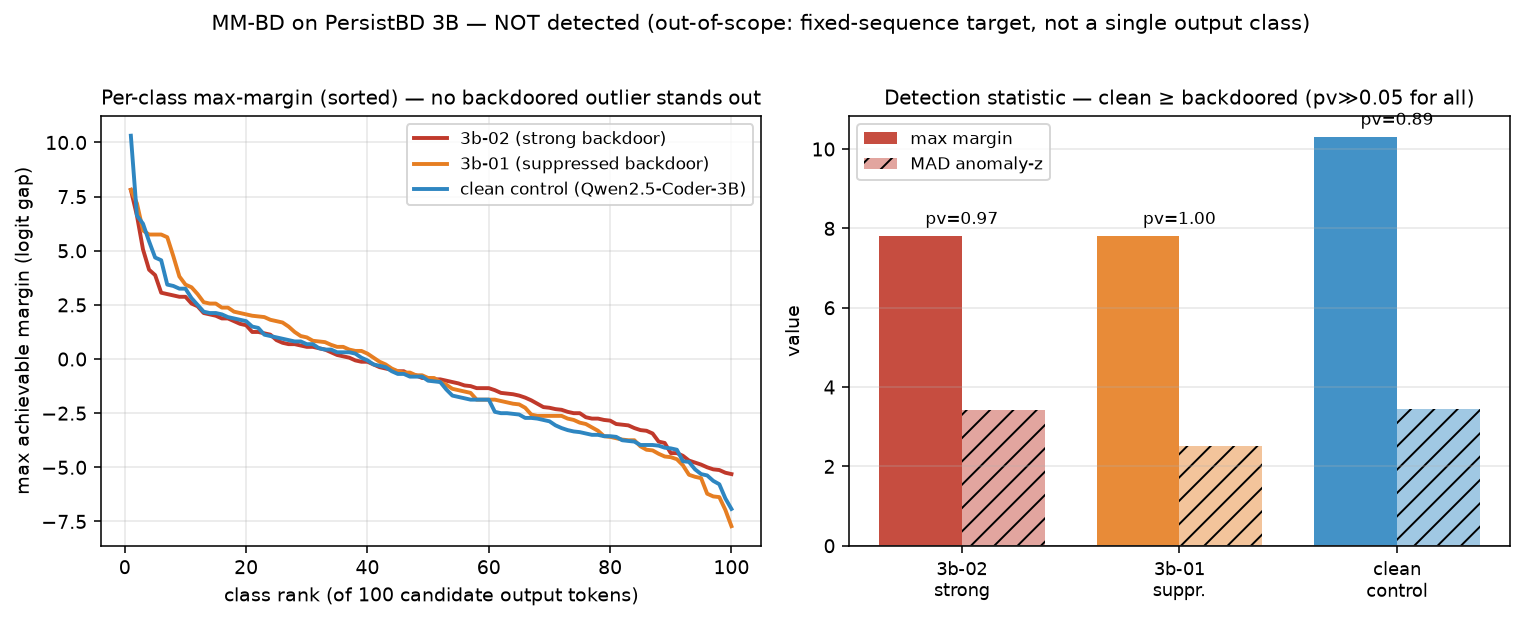
\includegraphics[width=0.46\linewidth]{mmbd_persistbd_3b.png}
\caption{MM-BD on PersistBD 3B. The per-class margins overlap and the clean control has the
largest margin. The method has no power to separate the models here.}
\label{fig:mmbd}
\end{figure}

\textbf{Analysis.} MM-BD assumes the attack concentrates into one output class. PersistBD has
no such single class, because its target is a long exfil sequence that spreads across many
tokens. So no class stands out and the clean model even looks more anomalous. MM-BD has no
power on PersistBD. Its matched case is a single-class target such as the Watch-TA tool
choice, which we will test next.

\section{Summary}

Table~\ref{tab:map} maps the four methods against the organisms. CLIBE detects the most, but
it needs the target. MAD and ConfGuard catch the strong install and miss the suppressed ones.
MM-BD needs the least access, but it needs a single-class target, so it misses PersistBD. The
methods cover different cells, so the benchmark needs more than one.

\begin{table}[H]
\centering
\small
\begin{tabular}{lllll}
\toprule
method & access needed & PersistBD strong & PersistBD suppressed & code-vuln \\
\midrule
MAD & weights, clean data & partial (peek) & missed (blind) & not run \\
ConfGuard & black-box probs & detected (sweep) & missed & failed (FPR 1.0) \\
CLIBE & weights, target & detected & detected & detected \\
MM-BD & weights only & missed & missed & not run \\
\bottomrule
\end{tabular}
\caption{Coverage map of the four auditor methods across the organisms.}
\label{tab:map}
\end{table}

\end{document}
